\documentclass[a4paper]{article}

%% Language and font encodings
\usepackage[english]{babel}
\usepackage[utf8x]{inputenc}
\usepackage[T1]{fontenc}

%% Sets page size and margins
\usepackage[a4paper,top=3cm,bottom=2cm,left=3cm,right=3cm,marginparwidth=1.75cm]{geometry}

%% Useful packages
\usepackage{amsmath}
\usepackage{graphicx}
\usepackage[colorinlistoftodos]{todonotes}
\usepackage[colorlinks=true, allcolors=blue]{hyperref}

\title{Benchmarking P2C for HPC}
\author{Joseph Anthony C. Hermocilla}

\begin{document}
\maketitle

\begin{abstract}
We report some results of benchmarking P2C for HPC using NPB 3.3.1.
\end{abstract}

\section{Introduction}
In order to evaluate the performance of P2C for applications, NPB Benchmark applications were tested. A 16-node cluster was deployed using vcluster.

\section{NPB Benchmark Applications}

\subsection{CG}

See the code for Figure \ref{fig:CG_A} in this section for an example.

%\begin{figure}
%\centering
%\includegraphics[width=0.3\textwidth]{frog.jpg}
%\caption{\label{fig:frog}This frog was uploaded via the project menu.}
%\end{figure}

\begin{figure}
\centering
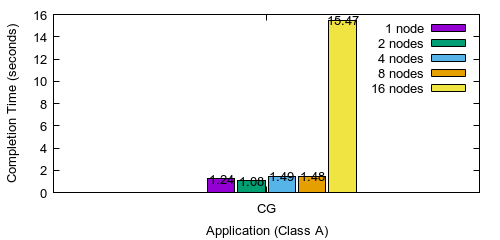
\includegraphics[width=0.8\textwidth]{figures/CG.A.png}
\caption{\label{fig:CG_A}This frog was uploaded via the project menu.}
\end{figure}

\begin{figure}
\centering
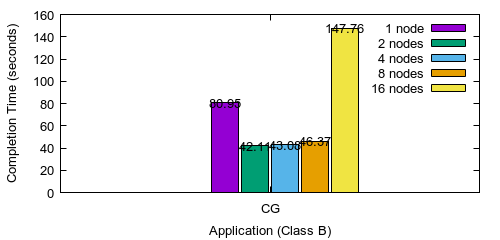
\includegraphics[width=0.8\textwidth]{figures/CG.B.png}
\caption{\label{fig:CG_B}This frog was uploaded via the project menu.}
\end{figure}



\bibliographystyle{alpha}
\bibliography{sample}

\end{document}